\PassOptionsToPackage{usenames,dvipsnames,table}{xcolor}
\documentclass[sigconf,balance,nonacm]{acmart}

\newcommand\tab[1][10mm]{\hspace*{#1}}
% packages
\usepackage[utf8]{inputenc}
\usepackage{amsmath}
\usepackage{commath}

\usepackage{graphicx}
\usepackage[caption=false,font=footnotesize]{subfig}
    
\usepackage{cleveref}

% algorithms
\usepackage{algorithm,algpseudocode}

\usepackage{listings} 
\usepackage{color}
\usepackage{soul}
\usepackage{booktabs}
\usepackage{multirow}
\usepackage[nolist,nohyperlinks]{acronym}
\usepackage{xspace}
\usepackage{url}
\usepackage{indentfirst}

\usepackage{siunitx}
\usepackage{float}
\usepackage{pgfplots}
\usepackage{pgfplotstable}

\pgfplotsset{
    width=8cm,
    height=5cm,
    xlabel={Matrix size},
    xmin=512, xmax=3072, xtick=data,
    ylabel={Runtime (\unit{\second})},
    ymin=0,
    legend pos=north west,
    tick label style={
        /pgf/number format/.cd,
        fixed,
        fixed zerofill=false,
        precision=5,
        scaled ticks=false,
        /tikz/.cd
    },
    compat=1.18
}

\definecolor{dkgreen}{rgb}{0,0.6,0}
\definecolor{gray}{rgb}{0.5,0.5,0.5}
\definecolor{mauve}{rgb}{0.58,0,0.82}
\definecolor{orange}{rgb}{.7,.3,0} 
\makeatletter
\lst@InstallKeywords k{types}{typestyle}\slshape{typestyle}{}ld
\makeatother
\lstset{
    language=c++,
    aboveskip=10pt,
    belowskip=10pt,
    showstringspaces=false,
    basicstyle={\small\ttfamily},
    keywordstyle=\color{blue},
    commentstyle=\color{dkgreen},
    stringstyle=\color{mauve},
    typestyle=\color{orange},
    breaklines=true,
    breakatwhitespace=true,
    postbreak=\mbox{\textcolor{red}{$\hookrightarrow$}\space},
    morekeywords={
        in, from, to
    },
    moretypes={
        range
    }
}

%Graphs and Table Configs
\pgfkeys{/pgf/number format/.cd,fixed,precision=4}
\pgfplotstableset{
    col sep=comma,
    clear infinite,
    empty cells with={\ensuremath{-}},
    every head row/.style={
        before row=\hline,
        after row=\hline\hline
    },
    display columns/0/.style={
        fixed,
        precision=0
    },
    every last row/.style={after row=\hline},
    every column/.style={column type/.add={|}{}},
    every first column/.style={column type/.add={|}{}},
    every last column/.style={column type/.add={}{||}},
    sci zerofill=true,
    fixed zerofill=true,
    precision=3,
}

%Table definitions
\pgfplotstableread[]{data/runtime.csv}\dataRuntime
\pgfplotstableread[]{data/gflops.csv}\dataGflops
\pgfplotstableread[]{data/l1.csv}\dataLone
\pgfplotstableread[]{data/l2.csv}\dataLtwo

% Reduce size between figures and text
\setlength{\textfloatsep}{10pt plus 1.0pt minus 2.0pt}
\setlength{\dbltextfloatsep}{10pt plus 1.0pt minus 2.0pt}
\setlength{\floatsep}{6pt plus 1.0pt minus 1.0pt}
\setlength{\dblfloatsep}{6pt plus 1.0pt minus 1.0pt}
\setlength{\intextsep}{6pt plus 1.0pt minus 1.0pt}

% document
\begin{document}

% title and authors
\title{Performance Evaluation for Single Threaded Matrix Multiplication Algorithms}

\author{\begin{tabular}{rl}
        \textbf{João Pereira}  & up202007145@fe.up.pt \\
        \textbf{Mariana Rocha} & up202004656@fe.up.pt \\
        \textbf{Matias Vaz}    & up201900194@fc.up.pt
    \end{tabular}}

\affiliation{%
    \institution{DEI, FEUP}
    \city{Porto}
    \country{Portugal}
}

\begin{abstract}

    This report was made in the context of the Parallel and Distributed Computing (CPD) course unit to solidify the course content with practice. The main goal of the project was to develop, compare, and document the code for matrix multiplication in single-threaded applications.

    The idea behind the practical work was to learn about the CPU performance impact of accessing large amounts of data in memory. Thus, we compared different algorithms with different ways to optimize memory access in C++ and Python.

\end{abstract}

\maketitle

% % % % % % % % % % % % % % % % % % % % %
% 			Problem Description}
% % % % % % % % % % % % % % % % % % % % %
\section{Problem Description}

The main problem for the project was evaluating the performance of different algorithms. The main difference for the given algorithms isn't the result itself, nor a math insight for general use, but a computation optimization for accessing the memory fewer times or in a faster manner.

For this study, three algorithms were used to evaluate the costs that different approaches would have on performance in a single-threaded environment. We recreated these algorithms in C++ and Python and compared different sizes for square matrices.

We chose these languages based on their current usage. Since C++ is a compiled fast-performance programming language also used for machine learning algorithms, which extensively use matrix multiplications. The other one is Python, a popular language for beginners in programming, with a more friendly and soft learning curve. It is also used extensively for data science problems, which use matrix multiplications.

% % % % % % % % % % % % % % % % % % % % %
% 	    Algorithms Explanation
% % % % % % % % % % % % % % % % % % % % %
\section{Algorithms Explanation}

\subsection{Naive Matrix Multiplication}

The naive matrix multiplication algorithm was provided in a C++ program and later our group implemented the same algorithm in the Python language.

The algorithm operates as follows: the result in the $i$-th row and $j$-th column of matrix $\mathbf{C}$ is the outcome of the dot product between the elements in the $i$-th row of matrix $\mathbf{A}$ and the $j$-th column of matrix $\mathbf{B}$. This results in a time complexity of $O(2n^3)$.

\begin{minipage}{\linewidth}
    \begin{lstlisting}
for i in range(0, matrix_size, 1):
  for j in range(0, matrix_size, 1):
    for k in range(0, matrix_size, 1):
      matrix_c[i][j] += matrix_a[i][k] * matrix_b[k][j]
\end{lstlisting}
\end{minipage}

\begin{figure}[H]
    \centering
    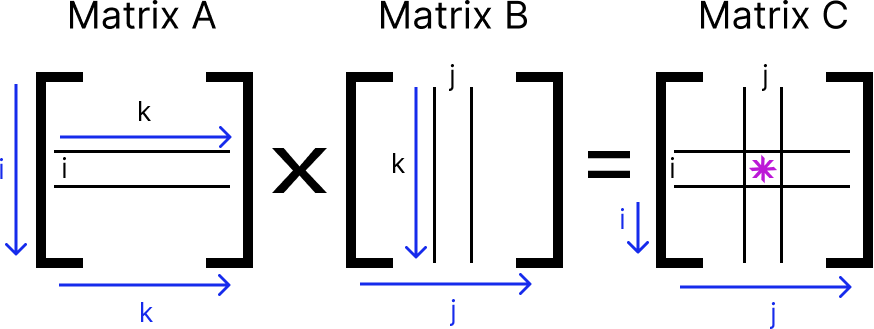
\includegraphics[width=0.8\columnwidth]{figures/naive.png}
    \caption{Naive Matrix Multiplication algorithm illustration}
    \label{fig:naive_illustration}
\end{figure}

\subsection{Lines Matrix Multiplication}

This algorithm differs from the one presented above in the order of the second and third \lstinline{for} loops.

The algorithm operates as follows: the result in the $i$-th row and $j$-th column of matrix $\mathbf{C}$ is also the outcome of the dot product between the elements in the $i$-th row of matrix $\mathbf{A}$ and the $j$-th column of matrix $\mathbf{B}$. It differs from the former because the whole dot product is not calculated at once. It multiplies an element of $\mathbf{A}$ with a row of $\mathbf{B}$, accumulating the result in the correct row of $\mathbf{C}$. This results in a time complexity of $O(2n^3)$.

\begin{minipage}{\linewidth}
    \begin{lstlisting}
for i in range(0, matrix_size, 1):
  for k in range(0, matrix_size, 1):
    for j in range(0, matrix_size, 1):
      matrix_c[i][j] += matrix_a[i][k] * matrix_b[k][j]
\end{lstlisting}
\end{minipage}

\begin{figure}[H]
    \centering
    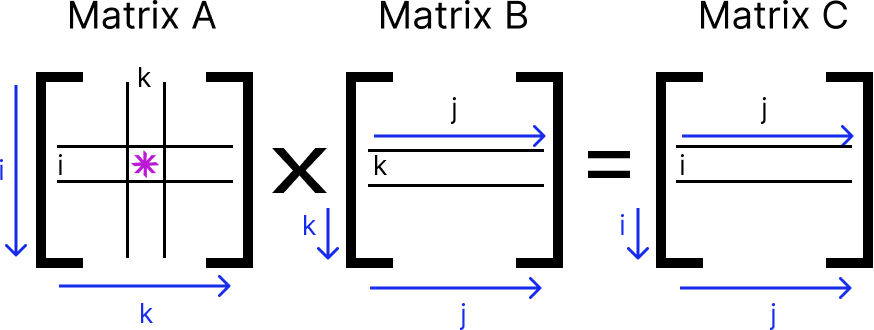
\includegraphics[width=0.8\columnwidth]{figures/lines.png}
    \caption{Lines Matrix Multiplication algorithm illustration}
    \label{fig:lines_illustration}
\end{figure}

\subsection{Block Matrix Multiplication}

The block matrix algorithm works as follows: firstly, both matrices to be multiplied are divided into blocks of size $s$, resulting in $n$ blocks. Those blocks are treated as elements of a matrix and the lines matrix multiplication algorithm is used to multiply them. This results in a time complexity of $O(2n^3)$.

\begin{minipage}{\linewidth}
    \begin{lstlisting}
for ib in range(0, n, 1):
  for kb in range(0, n, 1):
    for jb in range(0, n, 1):
      for i in range(ib * s, (ib + 1) * s, 1):
    	for k in range(kb * s, (kb + 1) * s, 1):
          for j in range(jb * s, (jb + 1) * s, 1):
            matrix_c[i][j] += matrix_a[i][k] * matrix_b[k][j]
\end{lstlisting}
\end{minipage}

\begin{figure}[H]
    \centering
    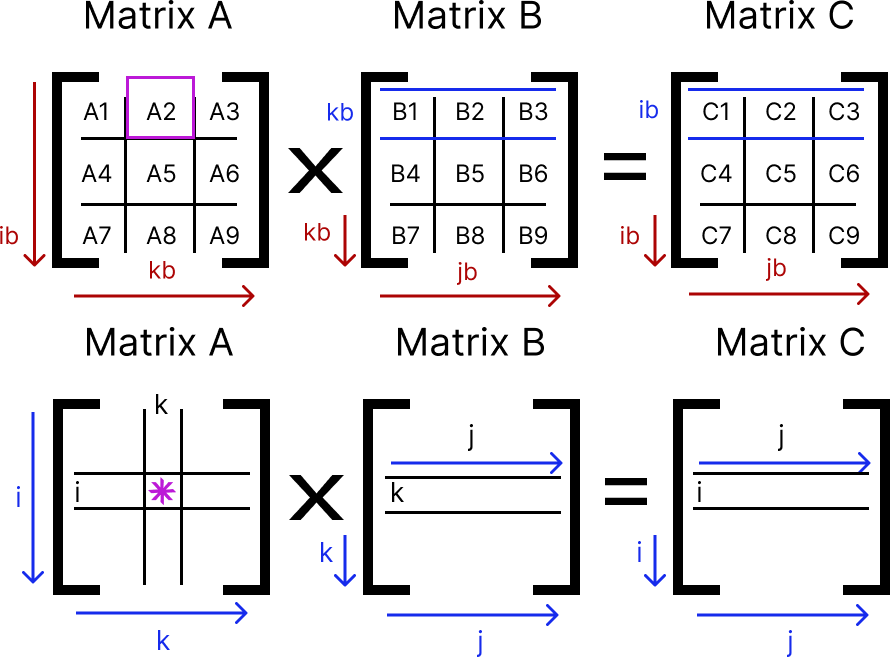
\includegraphics[width=0.8\columnwidth]{figures/block.png}
    \caption{Block Matrix Multiplication algorithm illustration}
    \label{fig:blocks_illustration}
\end{figure}

% % % % % % % % % % % % % % % % % % % % %
% 			EXPERIMENTAL EVALUATION
% % % % % % % % % % % % % % % % % % % % %
\section{Experimental Setup}

Since every different hardware has its own peculiarities, it's important to share the details of the setup used for this project. It's important to mention, even with being able to easily parallelize the code with some of our tools, we decided to focus only on single-thread applications. After that, we will discuss the experimental results found.

\subsection{Computer Environment Setup}

For every scenario, a desktop computer running Ubuntu 22.04 with \qty{32}{\giga\byte} of ram and an AMD Ryzen 5 5600x was used to process everything.
Besides the terminal, no other essential process was open, minimizing the noise of other programs in our data.

For collecting the data cache misses, we used the package PAPI 7.0.0, a Linux tool developed by the University of Tennessee.

\subsection{Code Environment Setup}

For programming, we used C++ 11 with GCC 11.3.0, Python 3.9.13, PyPy 7.3.9, and Numba  0.55.1.
We chose these tools because of their broad use. Pypy is a Just In Time compiler for Python, and Numba is a framework that compiles and allows easy parallelization of Python code, using GPUs or CPUs.
Both tools hugely speed up the runtime.

The decision for using all these tools was supported by the trade-off between effort in development versus performance.
Using more abstractions often results in an easier process to develop, but hurts the resulting performance.

\section{Experimental Results}

The experimental results were surprising.
Regardless of the gain in performance related to better memory access, we got some interesting results we'd like to point out.

First of all, the block algorithms didn't show any kind of improvement in performance in our tests. That wasn't our first assumption.
We could also notice all block sizes having relatively close runtimes.

In \ref{sub:basic} and \ref{sub:line}, we will compare the time performance between Python and C++, and will analyse the memory performance for C++.
In \ref{sub:block}, we will analyse the performance in C++ only.
And in \ref{sub:overall}, we will give a brief comparison between all the algorithms and languages.
You can find tables with all the results in the Appendix.

\subsection{Basic Multiplication Performance}
\label{sub:basic}

In figure \ref{fig:basic}, we can see how slow Python is compared to C++.
In a square matrix with size 3072, we got a runtime of \qty{4692.512}{\second}, versus \qty{149.787}{\second} for C++.
That means C++ had 31.32 times better performance.

You can also see the difference between C++ and the alternative Python implementations.
PyPy and C++ had similar performance in our tests, being capable of running with a size of 3072 in around \qty{150}{\second}.
The Numba code, without any kind of parallelization, is a little bit slower compared to the other two tools.

\begin{figure}[H]
    \centering
    \begin{tikzpicture}
        \begin{axis}[]
            \addplot[
                color=orange,
                mark=square
            ] table[x=n, y=P-N] {\dataRuntime};
            \addlegendentry{Python - Naive}

            \addplot[
                color=blue,
                mark=square
            ] table[x=n, y=C++-N] {\dataRuntime};
            \addlegendentry{C++ - Naive}

            \addplot[
                color=green,
                mark=square
            ] table[x=n, y=PP-N] {\dataRuntime};
            \addlegendentry{PyPy - Naive}

            \addplot[
                color=red,
                mark=square
            ] table[x=n, y=PN-N] {\dataRuntime};
            \addlegendentry{Numba - Naive}
            % \legend{S(FER; a)}
        \end{axis}
    \end{tikzpicture}
    \begin{tikzpicture}
        \begin{axis}[]
            \addplot[
                color=blue,
                mark=square
            ] table[x=n, y=C++-N] {\dataRuntime};
            \addlegendentry{C++ - Naive}

            \addplot[
                color=green,
                mark=square
            ] table[x=n, y=PP-N] {\dataRuntime};
            \addlegendentry{PyPy - Naive}

            \addplot[
                color=red,
                mark=square
            ] table[x=n, y=PN-N] {\dataRuntime};
            \addlegendentry{Numba - Naive}
        \end{axis}
    \end{tikzpicture}
    \caption{Runtime for the Basic algorithm}
    \label{fig:basic}
\end{figure}

\subsection{Lines Multiplication Performance}
\label{sub:line}

In figure \ref{fig:line}, we once again see how slow Python is compared to C++.
In a square matrix with size 3072, we got a runtime of \qty{3679.208}{\second}, versus \qty{10.874}{\second} for C++.
That means C++ had 338.35 times better performance.

You can also see the contrast between C++ and the alternative Python implementations.
PyPy had almost exactly the same performance as in \ref{sub:basic}, while C++ and Numba had better performance, with runtimes of around \qty{11}{\second} and \qty{40}{\second}, respectively.

\begin{figure}[H]
    \centering
    \begin{tikzpicture}
        \begin{axis}[]
            \addplot[
                color=orange,
                mark=square
            ] table[x=n, y=P-L] {\dataRuntime};
            \addlegendentry{Python - Lines}

            \addplot[
                color=blue,
                mark=square
            ] table[x=n, y=C++-L] {\dataRuntime};
            \addlegendentry{C++ - Lines}

            \addplot[
                color=green,
                mark=square
            ] table[x=n, y=PP-L] {\dataRuntime};
            \addlegendentry{PyPy - Lines}

            \addplot[
                color=red,
                mark=square
            ] table[x=n, y=PN-L] {\dataRuntime};
            \addlegendentry{Numba - Lines}
        \end{axis}
    \end{tikzpicture}
    \begin{tikzpicture}
        \begin{axis}[]
            \addplot[
                color=blue,
                mark=square
            ] table[x=n, y=C++-L] {\dataRuntime};
            \addlegendentry{C++ - Lines}

            \addplot[
                color=green,
                mark=square
            ] table[x=n, y=PP-L] {\dataRuntime};
            \addlegendentry{PyPy - Lines}

            \addplot[
                color=red,
                mark=square
            ] table[x=n, y=PN-L] {\dataRuntime};
            \addlegendentry{Numba - Lines}
        \end{axis}
    \end{tikzpicture}
    \caption{Runtime for the Lines algorithm}
    \label{fig:line}
\end{figure}

\subsection{Block Multiplication Performance}
\label{sub:block}

In figure \ref{fig:blocks}, it is possible to see the runtime for the Blocks algorith with different block sizes.
One interesting thing to notice is that the block size used had little to no impact on the overall performance.
This observation would probably change in parallelized code, but any predictions as to which size would be best would be pure conjecture, as there are many variables that could affect this outcome.

\begin{figure}[H]
    \centering
    \begin{tikzpicture}
        \begin{axis}[
                xmin=4096, xmax=10240,
            ]
            \addplot[
                color=blue,
                mark=square
            ] table[x=n, y=C++-B-128] {\dataRuntime};
            \addlegendentry{Block size = 128}

            \addplot[
                color=red,
                mark=square
            ] table[x=n, y=C++-B-256] {\dataRuntime};
            \addlegendentry{Block size = 256}

            \addplot[
                color=magenta,
                mark=square
            ] table[x=n, y=C++-B-512] {\dataRuntime};
            \addlegendentry{Block size = 512}

            \addplot[
                color=green,
                mark=square
            ] table[x=n, y=C++-B-1024] {\dataRuntime};
            \addlegendentry{Block size = 1024}
        \end{axis}
    \end{tikzpicture}
    \caption{Runtime for the Blocks algorithm}
    \label{fig:blocks}
\end{figure}

\subsection{Overall Comparison}
\label{sub:overall}

All tested algorithms were slower when using a Python implementation compared to C++.
This is due to the fact that Python is an interpreted language, which greatly increases the runtime for any algorithm.
When using PyPy, a Just In Time compiler, this performance hit largely goes away, but it is still slower than when using C++, as the compilation happens at runtime, and not earlier.
Interestingly, PyPy gains almost no performance when switching to the Lines algorithm, this could suggest that it optimizes the Naive algorithm by itself.
The Numba library for Python brought its performance much closer to C++ than PyPy, but still about four times slower.

Comparing the Naive algorithm with the Lines algorithm, all implementations get a speedup in performance.
This can be attributed to a better memory access strategy that minimizes cache misses, which are very expensive.
As seen in figures \ref{fig:l1cache} and \ref{fig:l2cache}, the Lines algorithm reduces L1 cache misses by an order of magnitude and L2 cache misses by up to three orders of magnitude in larger matrices.

\begin{figure}[H]
    \centering
    \begin{tikzpicture}
        \begin{axis}[
                xmax=10240, xtick={512, 2048, 4096, 6144, 8192, 10240},
                ylabel={Cache Misses},
                y tick label style={
                        scaled ticks=true,
                        /pgf/number format/relative*=9
                    }
            ]
            \addplot[
                color= orange,
                mark=square
            ] table[x=n, y=C++-N] {\dataLone};
            \addlegendentry{Naive}

            \addplot[
                color=yellow,
                mark=square
            ] table[x=n, y=C++-L] {\dataLone};
            \addlegendentry{Lines}

            \addplot[
                color=blue,
                mark=square
            ] table[x=n, y=C++-B-128] {\dataLone};
            \addlegendentry{Block size = 128}

            \addplot[
                color=red,
                mark=square
            ] table[x=n, y=C++-B-256] {\dataLone};
            \addlegendentry{Block size = 256}

            \addplot[
                color=magenta,
                mark=square
            ] table[x=n, y=C++-B-512] {\dataLone};
            \addlegendentry{Block size = 512}

            \addplot[
                color=green,
                mark=square
            ] table[x=n, y=C++-B-1024] {\dataLone};
            \addlegendentry{Block size = 1024}
        \end{axis}
    \end{tikzpicture}
    \begin{tikzpicture}
        \begin{axis}[
                xmax=10240, xtick={512, 2048, 4096, 6144, 8192, 10240},
                ylabel={Cache Misses},
                y tick label style={
                        scaled ticks=true,
                        /pgf/number format/relative*=9
                    }
            ]
            \addplot[
                color=yellow,
                mark=square
            ] table[x=n, y=C++-L] {\dataLone};
            \addlegendentry{Lines}

            \addplot[
                color=blue,
                mark=square
            ] table[x=n, y=C++-B-128] {\dataLone};
            \addlegendentry{Block size = 128}

            \addplot[
                color=red,
                mark=square
            ] table[x=n, y=C++-B-256] {\dataLone};
            \addlegendentry{Block size = 256}

            \addplot[
                color=magenta,
                mark=square
            ] table[x=n, y=C++-B-512] {\dataLone};
            \addlegendentry{Block size = 512}

            \addplot[
                color=green,
                mark=square
            ] table[x=n, y=C++-B-1024] {\dataLone};
            \addlegendentry{Block size = 1024}
        \end{axis}
    \end{tikzpicture}
    \caption{L1 data cache misses for C++ Algorithms}
    \label{fig:l1cache}
\end{figure}

\begin{figure}[ht!]
    \centering
    \begin{tikzpicture}
        \begin{axis}[
                xmax=10240, xtick={512, 2048, 4096, 6144, 8192, 10240},
                ylabel={Cache Misses},
                y tick label style={
                        scaled ticks=true,
                        /pgf/number format/relative*=9
                    }
            ]
            \addplot[
                color= orange,
                mark=square
            ] table[x=n, y=C++-N] {\dataLtwo};
            \addlegendentry{Naive}

            \addplot[
                color=yellow,
                mark=square
            ] table[x=n, y=C++-L] {\dataLtwo};
            \addlegendentry{Lines}

            \addplot[
                color=blue,
                mark=square
            ] table[x=n, y=C++-B-128] {\dataLtwo};
            \addlegendentry{Block size = 128}

            \addplot[
                color=red,
                mark=square
            ] table[x=n, y=C++-B-256] {\dataLtwo};
            \addlegendentry{Block size = 256}

            \addplot[
                color=magenta,
                mark=square
            ] table[x=n, y=C++-B-512] {\dataLtwo};
            \addlegendentry{Block size = 512}

            \addplot[
                color=green,
                mark=square
            ] table[x=n, y=C++-B-1024] {\dataLtwo};
            \addlegendentry{Block size = 1024}
        \end{axis}
    \end{tikzpicture}
    \begin{tikzpicture}
        \begin{axis}[
                xmax=10240, xtick={512, 2048, 4096, 6144, 8192, 10240},
                ylabel={Cache Misses},
                y tick label style={
                        scaled ticks=true,
                        /pgf/number format/relative*=9
                    }
            ]
            \addplot[
                color=yellow,
                mark=square
            ] table[x=n, y=C++-L] {\dataLtwo};
            \addlegendentry{Lines}

            \addplot[
                color=blue,
                mark=square
            ] table[x=n, y=C++-B-128] {\dataLtwo};
            \addlegendentry{Block size = 128}

            \addplot[
                color=red,
                mark=square
            ] table[x=n, y=C++-B-256] {\dataLtwo};
            \addlegendentry{Block size = 256}

            \addplot[
                color=magenta,
                mark=square
            ] table[x=n, y=C++-B-512] {\dataLtwo};
            \addlegendentry{Block size = 512}

            \addplot[
                color=green,
                mark=square
            ] table[x=n, y=C++-B-1024] {\dataLtwo};
            \addlegendentry{Block size = 1024}
        \end{axis}
    \end{tikzpicture}
    \caption{Cache misses on L2 for C++ Algorithms}
    \label{fig:l2cache}
\end{figure}

Cache misses are minimized because, as seen in figure \ref{fig:lines_illustration}, the inner loop does not change which row of the matrices we're accessing.
This is beneficial because our matrices are stored as a contiguous array in memory, with the rows next to each other, and CPUs pull contiguous blocks of memory into the cache at a time.
So "jumping around" in memory, as we do when changing rows, is very expensive in terms of memory access.

In figure \ref{fig:gflops}, we can see the resulting performance for each of the algorithms.
It stays mostly constant for each algorithm, except for small matrices.
Here the Naive algorithm is slightly faster, as the amount of cache misses is also smaller when compared to the computations themselves.
The Lines algorithm gets a bump around a matrix size of 1024, this is the point where our program reaches the best balance between smaller matrices, where overhead has a bigger impact, and larger matrices, where loading data from memory has a bigger impact.
The Blocks algorithm is slightly slower at smaller sizes, probably due to the overhead that comes with splitting those matrices unnecessarily.

\begin{figure}[H]
    \centering
    \begin{tikzpicture}
        \begin{axis}[
                xmax=10240, xtick={512, 2048, 4096, 6144, 8192, 10240},
                legend pos=north east,
                ylabel={Perfomance (\unit{\giga flop \per\second})}
            ]
            \addplot[
                color= orange,
                mark=square
            ] table[x=n, y=C++-N] {\dataGflops};
            \addlegendentry{C++ - Naive}

            \addplot[
                color=yellow,
                mark=square
            ] table[x=n, y=C++-L] {\dataGflops};
            \addlegendentry{C++ - Lines}

            \addplot[
                color=blue,
                mark=square
            ] table[x=n, y=C++-B-128] {\dataGflops};
            \addlegendentry{Block size = 128}

            \addplot[
                color=red,
                mark=square
            ] table[x=n, y=C++-B-256] {\dataGflops};
            \addlegendentry{Block size = 256}

            \addplot[
                color=magenta,
                mark=square
            ] table[x=n, y=C++-B-512] {\dataGflops};
            \addlegendentry{Block size = 512}

            \addplot[
                color=green,
                mark=square
            ] table[x=n, y=C++-B-1024] {\dataGflops};
            \addlegendentry{Block size = 1024}
        \end{axis}
    \end{tikzpicture}
    \caption{Performance of different algorithms}
    \label{fig:gflops}
\end{figure}

This chart reinforces what was said in previous sections, that the Lines algorithm is faster than the Naive algorith, and the Blocks algorithm is slightly slower than the Lines algorithm, at least in a single threaded application.

Additional data not pictured in these figures can be found in the Appendix.

% % % % % % % % % % % % % % % % % % % % %
% 			RELATED WORK
% % % % % % % % % % % % % % % % % % % % %
\section{Related Work}
\label{sec:rel}

In future work, we could parallelize the code using CPUs and GPUs and compare the different approaches.
The usage of multi-processing methods would be the main way to gain performance, which would provide a better understanding of the memory impact and performance possibilities.

Besides this, exploring more algorithms to eventually find an even more efficient one in terms of memory access could also be an option.

% % % % % % % % % % % % % % % % % % % % %
% 			CONCLUSIONS
% % % % % % % % % % % % % % % % % % % % %
\section{Conclusions}
\label{sec:conclusions}

This practical assignment was instrumental in a better understanding of the importance of efficiently accessing memory in programs according to their hardware design and its impact on overall performance.

It was also important for realizing just how much slower Python is compared to C++, and that there are faster alternatives that improve its performance without sacrificing its user-friendly characteristics, namely PyPy and Numba.

To conclude, choosing the most performant algorithm goes further than complexity analysis.
Thinking about the programming language, the hardware and the specific application of the algorithm is also important.
In some areas, such as machine learning or scientific research, differences like these that may seem small can have a big difference, as they work with large amounts of data and low latency is a critical requirement.

% % % % % % % % % % % % % % % % % % % % %
% 			ACKNOWLEDGMENTS
% % % % % % % % % % % % % % % % % % % % %
\section*{Acknowledgments}

We want to thank all the staff of the Parallel and Distributed Computing course unit, especially our practical lesson teacher, Carlos Baquero-Moreno.

% % % % % % % % % % % % % % % % % % % % %
% 			APPENDIX
% % % % % % % % % % % % % % % % % % % % %
\onecolumn
\appendix
\section{Appendix}
\label{appendix}

\begin{table}[H]
    \centering
    \pgfplotstabletypeset[
    columns/n/.style={column name={}},
    columns/C++-N/.style={column name={}},
    columns/C++-L/.style={column name={}},
    columns/C++-B-128/.style={column name={128}},
    columns/C++-B-256/.style={column name={256}},
    columns/C++-B-512/.style={column name={512}},
    columns/C++-B-1024/.style={column name={1024}},
    columns/P-N/.style={column name={}},
    columns/P-L/.style={column name={}},
    columns/PP-N/.style={column name={}},
    columns/PP-L/.style={column name={}},
    columns/PN-N/.style={column name={}},
    columns/PN-L/.style={column name={}},
    every head row/.style={
            before row={
                    \hline
                    &
                    \multicolumn{6}{c|}{C++} &
                    \multicolumn{2}{c|}{Python} &
                    \multicolumn{2}{c|}{PyPy} &
                    \multicolumn{2}{c||}{Numba} \\
                    Matrix size & Naive & Lines &
                    \multicolumn{4}{c|}{Blocks} &
                    Naive & Lines &
                    Naive & Lines &
                    Naive & Lines \\
                },
            after row=\hline,
        },
    ]{\dataRuntime}
    \caption{Runtime for all algorithms (\unit{\second})}
    \label{table:runtime}
\end{table}

\begin{table}[H]
    \centering
    \pgfplotstabletypeset[
    columns/n/.style={column name={}},
    columns/C++-N/.style={column name={}},
    columns/C++-L/.style={column name={}},
    columns/C++-B-128/.style={column name={128}},
    columns/C++-B-256/.style={column name={256}},
    columns/C++-B-512/.style={column name={512}},
    columns/C++-B-1024/.style={column name={1024}},
    columns/P-N/.style={column name={}},
    columns/P-L/.style={column name={}},
    columns/PP-N/.style={column name={}},
    columns/PP-L/.style={column name={}},
    columns/PN-N/.style={column name={}},
    columns/PN-L/.style={column name={}},
    every head row/.style={
            before row={
                    \hline
                    &
                    \multicolumn{6}{c|}{C++} &
                    \multicolumn{2}{c|}{Python} &
                    \multicolumn{2}{c|}{PyPy} &
                    \multicolumn{2}{c||}{Numba} \\
                    Matrix size & Naive & Lines &
                    \multicolumn{4}{c|}{Blocks} &
                    Naive & Lines &
                    Naive & Lines &
                    Naive & Lines \\
                },
            after row=\hline,
        },
    ]{\dataGflops}
    \caption{Efficiency all algorithms (\unit{\giga flop \per \second})}
    \label{table:efficiency}
\end{table}

\begin{table}[H]
    \centering
    \pgfplotstabletypeset[
    columns/n/.style={column name={}},
    columns/C++-N/.style={column name={}},
    columns/C++-L/.style={column name={}},
    columns/C++-B-128/.style={column name={128}},
    columns/C++-B-256/.style={column name={256}},
    columns/C++-B-512/.style={column name={512}},
    columns/C++-B-1024/.style={column name={1024}},
    every head row/.style={
            before row={
                    \hline
                    Matrix size & Naive & Lines &
                    \multicolumn{4}{c||}{Blocks} \\
                },
            after row=\hline,
        },
    sci,
    ]{\dataLone}
    \caption{L1 data cache misses for C++ algorithms}
    \label{table:lone}
\end{table}

\begin{table}[H]
    \centering
    \pgfplotstabletypeset[
    columns/n/.style={column name={}},
    columns/C++-N/.style={column name={}},
    columns/C++-L/.style={column name={}},
    columns/C++-B-128/.style={column name={128}},
    columns/C++-B-256/.style={column name={256}},
    columns/C++-B-512/.style={column name={512}},
    columns/C++-B-1024/.style={column name={1024}},
    every head row/.style={
            before row={
                    \hline
                    Matrix size & Naive & Lines &
                    \multicolumn{4}{c||}{Blocks} \\
                },
            after row=\hline,
        },
    sci,
    ]{\dataLtwo}
    \caption{L2 data cache misses for C++ algorithms}
    \label{table:ltwo}
\end{table}

\end{document}
